\chapter{Model assumptions}

\section{Model assumptions revisited}

And this point you should understand 
\begin{itemize}
\item The mathematical definition of a linear regression model, as well as the assumptions that are being made. 
\item How to fit regression models in python.
\item How to interpret the results, including $R^2$, standard errors, confidence intervals and $p$-values. 
\end{itemize}
This is only half of data science (or as I like to call it, science). The other half involves 
\begin{itemize}
\item Building the ``right" model to answer a given scientific question 
\item Integrating prior knowledge into the model and inference  
\item identifying deficiencies in our models 
\item and changing to them to answer the scientific questions we are interested in
\end{itemize}


\subsection{General assumptions in statistical inference}

Whenever we build a model and perform statistical inference, we are making assumptions about the the data. We've discussed a few of the assumptions we make in linear regression models, but in this section we are going to take a deeper dive into regression modeling assumptions. Some of them are explicit assumptions of the linear regression model, while others are more general assumptions we make in statistical analysis which are buried underneath the model itself, and often overlooked. We start by discussing these assumptions. 

{\dfn Validity}:
We assume that data is actually relevant to your research objective. For example, someones income does not necessarily tell you about someones total assets (they have a lot of debt, or simply be terrible at managing their money). So studying income can be misleading for certain research questions. 
This is often an issue when we study response variables that are aggregate statistics, such as metrics of performance. Do the aggregate statistics actually predict the results we are interested in? It's also an issue with subjective traits, like wellbeing, happiness. We might be able to find what factors are associated with someone reporting they are happy on a survey, but do these factors actually predict someone's long term happiness?

{\dfn Representativeness}: Whenever we fit a model on a finite data set and use it to make predictions about samples outsite the data set (e.g. future elections). We are assuming our sample is representative of the entire population (or at least the subset of the population we are interested in making predictions about).  For example, if we fit a model using data from college basketball, will that same model be able to make predictions about the NBA? Maybe. If we can make predictions about elections in US, will we be able to predict the outcome of elections in the UK? Probably not. 

\subsection{Linear regression model assumptions}


%A central question we encounter when building an evaluating models: is what assumptions are appropriate? Thus, it is worth revisiting the model assumptions for a linear regression model. They are as follows
%\begin{enumerate}
%\item The distribution of $Y$ conditioned on $X$ is Normal with a mean that depends linearly on each $X_i$.
%\item Conditioned on $X$, the $Y$ values are independent and have equal variance. 
%\end{enumerate}
%
%In these notes, we explore the various ways model assumptions break down, how to detect them, and how the linear regression model can be extended to accommodate the deficiencies. 


Below we will grow through our modeling assumptions in the linear regression context. It's important recognize that all these assumptions are {\bf always false}. The question we must ask is whether they are adequate approximations for the questions we are interested in. If not, we need to understand how the data can be reorganized in a way that makes the linear regression model appropriate. 





%\section{ Equal standard deviation of errors}
%
%We assume that the standard deviations are not dependent on the values of the predictors. Fore example, when modeling kid's test scores we have assumed that the variation in test scores among students whose mothers attended high school is the same as the variation among students whose mothers did not. This assumption usually doesn't matter too much, 




\section{Normality of errors}



We assume that the distribution of the errors is Normal. Why do we make this assumption? Partly for convenience as it's easy to work with Normal distributions, but on a deeper level, normal distributions emerge when noise is due to the additive contributions of many small sources of randomness.  Mathematical, this is due to the central limit theorem. Roughly speaking, the Central limit theorem tells us that when noise is due to adding up many small source of randomness, we get a Normal distribution. 

\subsection{Missing a binary predictor}
Consider for example adult male or female height $h$. Neglecting environmental factors, we can think of someone's height as being determined by their gnome:
\begin{equation}
h = \bar{h} + \sum_i \alpha_i g_i 
\end{equation}
where $\alpha_i$ is the effect of a mutation of the $i$th gene and $g_i$ is $0$ if a person has a mutation and $1$ if not. There are tens of thousands of genes, so the central limit theorem tells us $h$ has a Normal distribution. This is what we would call a toy model, meaning that it is not meant to actually describe the distribution of height quantitatively, rather, it serves to help us understand why something like height will have a Normal distribution. 

On the other hand, if $h$ is the height of {\bf any} person, then 
\begin{equation}
h = x_{\rm male}\bar{h}_{\rm male} + (1-x_{\rm male})\bar{h}_{\rm female} + \sum_i \alpha_i g_i 
\end{equation}
Among *all* humans height will not have a Normal distribution because one particular factor, sex, has a very large effect. 

So we can model height using a linear regression model with normal errors **as long as we include sex as a predictor.** In this case, our regression model is 
\begin{equation}
h = ax_{\rm male} + b + \epsilon
\end{equation}
where
\begin{align}
a &= \bar{h}_{\rm male} - \bar{h}_{\rm female}\\
b &= \bar{h}_{\rm female}\\
\epsilon &= \sum_i \alpha_i g_i 
\end{align}


Normal noise also cannot model binary outcomes

{\bf If we want to model height as the response variable in a regression model we need to include sex as a predictor}



\subsection{Multiplicative randomness}
Let's first work with a simple example involving one predictor: the effect of height on earnings.

\begin{example}
\href{https://colab.research.google.com/drive/1bBeb3k5xEjGInFtjhB7X8B0LXqkGI0Tn#scrollTo=YGx6p6IPsIqA&line=1&uniqifier=1}{Problems with earnings model}
\end{example}

Why is the assumptions of normality problematic for earnings? This is a situation where a ``toy mode" can be very useful. A toy model for earnings is as follows. This model is not meant to have anything to do with the actual distribution of salaries, its only purpose is to illustrate a conceptual point that probably applies to the real distribution of salaries. 


Let's imagine $1000$ people {\bf of the same height} enter the workforce at the same time each with a starting salary of $y_0$k. $20$ years later there will of course be some variation in their earnings, represented by $\epsilon$ in the model. Let's think about what exactly causes that and the kind of distribution it might lead to. 

A person might get lucky and gets a promotion, or is hired into a very prestigious position and so their salary will increase to say $2y_0$. Raises are generally some percent of a person's salary, so now if this person continues to be successful in their career, their salary will increase by an amount proportional to $2y_0$. After $20$ years, the randomness in everyone's earning {\bf will not simply be the sum of many small factors.} 

To be mathematically precise, if someones gets a promotion that increases their salary by a factor $\phi_1$ after their first year on the job, their salary the next year will be 
\begin{equation}
y_1 = y_0\times \phi_1
\end{equation}
If they get a promotion after their second year that increase their salary by a factor $\phi_2$, their salary will be 
\begin{equation}
y_2 = y_1 \times \phi_2 = y_0 \times \phi_1 \times \phi_2
\end{equation}


If someones get's 20 promotions over 20 years which increase their salary by factors $\phi_1,\phi_2,\dots$ percent, their earning after $10$ years will be:
\begin{equation}
y = y_0\times \phi_1 \times \phi_2 \cdots \times \phi_{20}
\end{equation}


Now let's simulate the salaries of $1000$ people all get some sort of promotation or demotion each year. We will assume there is some variation in their promotions which we model by a Normal distribution:
\begin{equation}
\phi_i \sim {\rm Normal}(1.01,0.1)
\end{equation}
This says that, on average, someone's salary goes up by $1\%$, but it could increase or decrease by as much as $\approx 20\%$.

\begin{example}
\href{https://colab.research.google.com/drive/1bBeb3k5xEjGInFtjhB7X8B0LXqkGI0Tn#scrollTo=YGx6p6IPsIqA&line=1&uniqifier=1}{Earnings toy model}
\end{example}

This example illustrates how non-normality can arrises from multiplicative effects. Recall that logarithms have the effect of transforming products into sums, thus: 
\begin{equation}
\ln y = \ln y_0 + \sum_i \ln \phi_i 
\end{equation}
Intuitively, when we take the logarithm we are measuring our response variable in powers of $e$, or whatever the base of our log is (it doesn't matter). 



\begin{figure}[h]
    \centering
    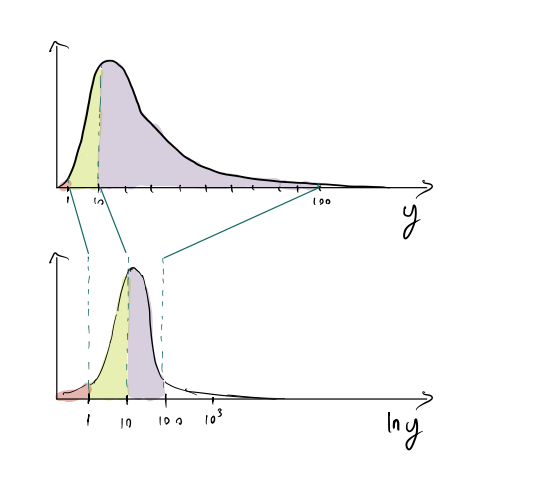
\includegraphics[width=0.8\textwidth]{log_hist}
    \caption{The effect of a log transform on the histogram for a very skewed distribution }
    \label{fig:log_hist}
\end{figure}

 

\subsection{Working on a log scale}
Now back to our regression model. It makes more sense to model earnings on a log scale:
\begin{equation}
\ln Y = a X + b + \epsilon
\end{equation}
where $X$ is height. What $a$ mean in terms of conditional averages? $a$ is the average difference in {\bf log earnings} between two people who differ in height by $1$ inch. When we think about differences in the log of a response variable, we should remember that
\begin{equation}
\ln Y_1 - \ln Y_2 = \ln Y_1/Y_2. 
\end{equation}
so differences in log earnings correspond to log ratios between earnings. 

We can also see this by exponentiating both sides of the linear regression equations. This yields
\begin{equation}
Y = e^{a X} e^b e^{\epsilon}
\end{equation}
The conditional average value of $y$ is 
\begin{equation}
\E[Y|X] = e^{a X} e^b \E[e^{\epsilon}]
\end{equation}
That is, our model is saying that {\bf if a person is one inch taller than someone else, they will make, on average, $e^{a}$ times as much money}

If $a$ is small (roughly between $-0.4$ and $0.4$), then a useful approximation is 
\begin{equation}
e^{a} \approx 1 + a. 
\end{equation}
Thus, {\bf if a person is one inch taller than someone else, they make on average about $100|a|\%$ more (or less) money, assuming $a$ is not too large}


\begin{example}
\href{https://colab.research.google.com/drive/1bBeb3k5xEjGInFtjhB7X8B0LXqkGI0Tn?usp=sharing}{Earnings}
\end{example}

\begin{example}
\href{https://colab.research.google.com/drive/1bBeb3k5xEjGInFtjhB7X8B0LXqkGI0Tn?usp=sharing}{Covid cases}
\end{example}


\section{Independence of errors}

In linear regression models, we generally assume the {\bf errors} or noise values $\epsilon_i$ are independent.
This assumption often fails when our predictor variables represent either time or space. The following example illustrates this. 


%Another example where this assumption is very often violated is time series. Let's say the average temperature on Hanover in is 50F in October. If one year it is particularly cold, say around 40F for most of the month {\bf this changes what we expect the temperature in November to deviate from the average}.


\begin{example}
\href{https://colab.research.google.com/drive/1bBeb3k5xEjGInFtjhB7X8B0LXqkGI0Tn?usp=sharing}{Linear regression on unemployment data}
\end{example}

\begin{exercise}
\href{https://colab.research.google.com/drive/1bBeb3k5xEjGInFtjhB7X8B0LXqkGI0Tn?usp=sharing}{Simulating time series model for unemployment}
\end{exercise}




\section{Residual plots}

The previous examples illustrate how the residuals can be used to evaluate the linear regression model assumptions. Indeed, residual plots are central tool used to access modeling assumptions; however, there are some subtle aspects to their interpretation, particularly when working with multiple predictors. Let's take a mode systematic look at the use of residual plots. 

The basic idea of residual plots is that by plotting the difference between the observed $y$ values and the prediction of the $\E[Y|X]$, or 
\begin{equation}
r_j  = Y_j - \sum_i^{K} \hat{a}_iX_{i,j},
\end{equation}
we can identify any patterns that would suggest the assumption of the linear regression model are violated. In the instance of a single-predictor, we can simply plot $r_j$ as a function of the predictor $X$. If we notice that the residuals do not appear to follow a normal distribution, or that the variance and mean change, then we should be skeptical.


 When we have multiple predictors, what do we plot on the $x$ axis? The answer is to plot $r_j$ as a function of the predictors value of $\E[Y|X]$, or $\sum_i^{K} \hat{a}_iX_{i,j}$. The following example illustrates why. 


\begin{example}
\href{https://colab.research.google.com/drive/1bBeb3k5xEjGInFtjhB7X8B0LXqkGI0Tn#scrollTo=Wt-Irm_AeY17&line=1&uniqifier=1}{Residual plots with multiple predictors}
\end{example}


\begin{figure}[h]
    \centering
    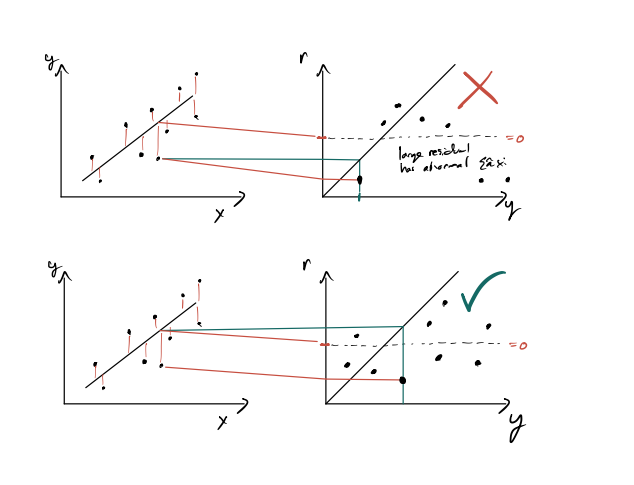
\includegraphics[width=0.8\textwidth]{res}
    \caption{Correct and incorrect way to plot residuals against response variable }
    \label{fig:res}
\end{figure}


\subsection{Identifying interactions in residual plots}


In regression models, we assume that the response variable is, on average, a linear function of each of the predictors. Here we focus on ``weak" nonlinearity, which comes from interactions between predictors rather than nonlinear dependence on the predictors themselves. 

To understand what we mean by {\dfn interactions}, consider the model 
\begin{align}
Y &= a_1X_1 + a_2X_2 + a_{1,2}X_1X_2 + \epsilon \\
\epsilon &\sim {\rm Normal}(0,\sigma_{\epsilon}).
\end{align}
This is technically not a linear regression model in the predictors $X_2$ and $X_2$ because of the term involving $X_1X_2$. The coefficient $a_{1,2}$ is called an interaction coefficient. How should we interpret this? First note that for fixed $X_2$ (respectively $X_1$), $Y$ is a linear function of $X_1$ (respectively $X_2$). If we group the terms involving $X_1$, we can see what the $Y$ vs. $X_1$ slope is for fixed $X_2$: 
\begin{equation}
Y = (a_1 + a_{1,2}X_2)X_1 + a_2 X_2 +  \epsilon
\end{equation}
Thus 
\begin{equation}
\tilde{a}_1(X_2) = a_1 + a_{1,2}X_2
\end{equation}
is a {\bf $X_2$ dependent slope}. We can now see the meaning of $a_{1,2}$: is the average increase in the conditional slope of $Y$ vs. $X_1$ corresponding an increase in $X_2$ by $1$. We could have done the same calculation with $X_1$ and $X_2$ swapped though, so there is an equivalent interpretation in terms of the slope of $Y$ vs. $X_2$. 



\begin{example}
\href{https://colab.research.google.com/drive/1bBeb3k5xEjGInFtjhB7X8B0LXqkGI0Tn?usp=sharing}{Identifying an interaction}
\end{example}


\begin{example}
\href{https://colab.research.google.com/drive/1bBeb3k5xEjGInFtjhB7X8B0LXqkGI0Tn#scrollTo=brPdGI7K9-7h&line=3&uniqifier=1}{Slopes in regression model with interaction terms?}
\end{example}


\begin{exercise}
\href{https://colab.research.google.com/drive/1bBeb3k5xEjGInFtjhB7X8B0LXqkGI0Tn#scrollTo=kTHIvvZba6ai&line=1&uniqifier=1}{Interpreting residual plots}
\end{exercise}









